%%%%%%%%%%%%%%%%%%%%%%%%%%%%%%%%%%%%%%%%%
% Beamer Presentation
% LaTeX Template
% Version 1.0 (10/11/12)
%
% This template has been downloaded from:
% http://www.LaTeXTemplates.com
%
% License:
% CC BY-NC-SA 3.0 (http://creativecommons.org/licenses/by-nc-sa/3.0/)
%
%%%%%%%%%%%%%%%%%%%%%%%%%%%%%%%%%%%%%%%%%

%----------------------------------------------------------------------------------------
%	PACKAGES AND THEMES
%----------------------------------------------------------------------------------------

\documentclass[aspectratio=169]{beamer}
\usepackage[utf8]{inputenc}
\usepackage{booktabs}
\usepackage{graphicx}
\usepackage{array}
\usepackage{caption}
\usepackage{threeparttable}
\usepackage{lscape}
\usepackage{import}
\usepackage{amsmath}
\usepackage{csvsimple}
\usepackage{siunitx}
\usepackage{subfigure}
\usepackage{filecontents}
\newenvironment{wideitemize}{\itemize\addtolength{\itemsep}{10pt}}{\enditemize}
\usepackage{appendixnumberbeamer}
\usepackage{float}
\usepackage{amsmath}  
\usepackage{tikz,pgfplots}
\usepackage{tkz-fct}
\usepackage{amsthm}
\pgfplotsset{compat=1.10}
\usepgfplotslibrary{fillbetween}
\newcommand{\vertLineFromPoint}[1]{
  \draw[dashed] 
  (#1) -- (#1|-{rel axis cs:0,0})
}
\newcommand{\horLineFromPoint}[1]{
  \draw[dashed] 
  (#1) -- (#1-|{rel axis cs:0,0})
}
\mode<presentation> {
\AtBeginSection[]
{
    \begin{frame}
        \frametitle{Table of Contents}
        \tableofcontents[currentsection]
    \end{frame}
}
% The Beamer class comes with a number of default slide themes
% which change the colors and layouts of slides. Below this is a list
% of all the themes, uncomment each in turn to see what they look like.

%\usetheme{default}
%\usetheme{AnnArbor}
%\usetheme{Antibes} -
%\usetheme{Bergen}
%\usetheme{Berkeley}
%\usetheme{Berlin}
\usetheme{Boadilla}
%\usetheme{CambridgeUS}
%\usetheme{Copenhagen} -
%\usetheme{Darmstadt}
%\usetheme{Dresden}
%\usetheme{Frankfurt}
%\usetheme{Goettingen}
%\usetheme{Hannover}
%\usetheme{Ilmenau}
%\usetheme{JuanLesPins}
%\usetheme{Luebeck}
%\usetheme{Madrid}
%\usetheme{Malmoe}
%\usetheme{Marburg}
%\usetheme{Montpellier}
%\usetheme{PaloAlto}
%\usetheme{Pittsburgh}
%\usetheme{Rochester} -
%\usetheme{Singapore}
%\usetheme{Szeged}
%\usetheme{Warsaw}

% As well as themes, the Beamer class has a number of color themes
% for any slide theme. Uncomment each of these in turn to see how it
% changes the colors of your current slide theme.

%\usecolortheme{albatross}
%\usecolortheme{beaver}
%\usecolortheme{beetle}
%\usecolortheme{crane}
%\usecolortheme{dolphin}
%\usecolortheme{dove}
%\usecolortheme{fly}
%\usecolortheme{lily}
%\usecolortheme{orchid}
%\usecolortheme{rose}
%\usecolortheme{seagull}
%\usecolortheme{seahorse}
%\usecolortheme{whale}
%\usecolortheme{wolverine}

%\setbeamertemplate{footline} % To remove the footer line in all slides uncomment this line
\setbeamertemplate{footline}[frame number] % To replace the footer line in all slides with a simple slide count uncomment this line
\setbeamertemplate{theorems}[numbered]
\setbeamertemplate{navigation symbols}{} % To remove the navigation symbols from the bottom of all slides uncomment this line
}
\setbeamertemplate{caption}{\raggedright\insertcaption\par}
  \setbeamertemplate{enumerate items}[default]
\usepackage{graphicx} % Allows including images
\usepackage{booktabs} % Allows the use of \toprule, \midrule and \bottomrule in tables
%\usepackage {tikz}
\newtheorem*{theorem*}{Theorem}
\newtheorem*{lemma*}{Lemma}
\newtheorem*{proposition}{Proposition}
\newtheorem*{corollary*}{Corollary}
\newtheorem*{definition*}{Definition}
\DeclareMathOperator*{\argmin}{arg\,min}
\newtheorem*{assumption}{Assumption}
\usetikzlibrary {positioning}
%\usepackage {xcolor}

%----------------------------------------------------------------------------------------
%	TITLE PAGE
%----------------------------------------------------------------------------------------

\title[Spatial]{Lecture 5: Spatial Competition and Product Differentiation} % The short title appears at the bottom of every slide, the full title is only on the title page

\author{Jacob Kohlhepp} % Your name
\institute[UCLA] % Your institution as it will appear on the bottom of every slide, may be shorthand to save space
{
Econ 101 \\ % Your institution for the title page
\medskip
}
\date{\today} % Date, can be changed to a custom date

\begin{document}

\begin{frame}
\titlepage % Print the title page as the first slide
\end{frame}

\begin{frame}{Introduction}
\begin{wideitemize}
    \item In Cournot and Bertrand we assumed firms sold identical products. 
    \item Sometimes this is a decent assumption. When is it not?\pause
    \item Lots of examples: cars, news coverage, political parties, etc.
    \item This opens up other dimensions for competition.
    \item Could be location, quality, color, attributes, etc.
\end{wideitemize}

\end{frame}

\begin{frame}{Product Differentiation}

\begin{wideitemize}
    \item It is actually hard to define what it means for products are differentiated.
    \item For the sake of this class, I will use this definition.
    \begin{definition}
    A market features \textbf{product differentiation} if there is an aspect of a good other than price that enters consumers' utility.
    \end{definition}
    \item This can be an attribute: like car color or toothpaste additives.
    \item It can also be something less tangible like ``quality" (reputation or prestige of the brand) or partisanship (of a news channel).
\end{wideitemize}

    
\end{frame}


\begin{frame}{Bertrand with Product Differentiation}
The following example is adapted from N\&S Example 15.4.
\begin{wideitemize}
    \item Google produces Android and Apple produces iOS. The software licenses are demanded by phone manufacturers and are substitutes.
    \item Demand for each is given by:
    \[q_i = a_i - p_i + p_{-i}/2\]
    \item The software has a fixed cost to invent of $C$ but has 0 cost per license.
    \item We can interpret the positive coefficient on price as reflecting the fact that the goods are substitutes.
    \item $a_i$ reflects unique attributes of each operating system that shift up demand.
    \item Firms compete in prices ($0\leq p_i \leq \infty$). Find a nash equilibrium (see handwritten notes)
\end{wideitemize}
    
\end{frame}


\begin{frame}{Interpreting Bertrand with Differentiation}

\begin{wideitemize}
    \item Remember that in regular Bertrand, $p=MC$ and we achieve perfect competition. With unit costs of production, this means 0 profit.
    \item Now look at profit when we add differentiation:
\[\pi_i^* = \bigg (\frac{8}{15}a_i + \frac{2}{15} a_{-i} \bigg )^2-C\]
\item How does profit change as we raise $a_{-i}$?\pause
\item Intuition: Greater demand for competitor's product (through attribute differences) results in competitor increasing price, which allows me to increase price.
\item Broader intuition: Product differentiation can help reduce competition and raise profit.
\end{wideitemize}


\end{frame}

\begin{frame}{Spatial Competition is Product Differentiation}
    \begin{columns}[T] % align columns
\begin{column}{.63\textwidth}
\begin{wideitemize}
    \item We can think of spatial competition as product differentiation.
    \item The location of a store determines who pays a transport cost to get there.
    \item Have you ever wondered why gas stations locate across the street from each other?
    \item We will eventually answer this question.
\end{wideitemize}
\end{column}%
\hfill%
\begin{column}{.34\textwidth}
\resizebox{\textwidth}{!}{
  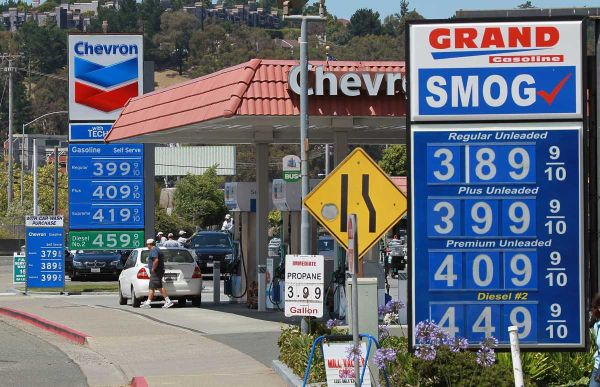
\includegraphics{6a00d8348f5cec53ef01b7c775228f970b.jpg}
  
}
\end{column}%
\end{columns}

  \hfill Source: Ghetty
\end{frame}

\begin{frame}{Hotelling Model}

\begin{wideitemize}
    \item \textbf{Players.} Two hot dog stands (A and B) on Santa Monica pier with predetermined locations (for now).
    \item Model the pier as a line segment of length $L$. Locations denoted as $a$ and $b$.
    \item We assume $A$ is to the left, $B$ is to the right.
    \item Consumers are uniformly located on the pier.
    \item Utility for a consumer at location $x$ of a hotdog from location $l$ and price $p$:
    \[u_l = v -p-t(x-l)^2\]
    \item Notice that if $t=0$ this is just the Bertrand model!
    \item What price is charged in equilibrium? (After graph, see handwritten notes)
\end{wideitemize}

\end{frame}

\begin{frame}{Solving Hotelling}
    \resizebox{\textwidth}{!}{
  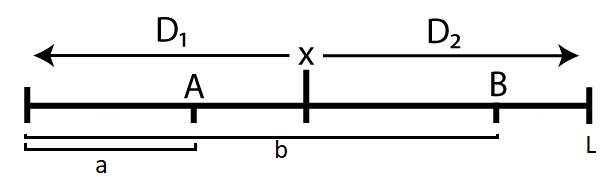
\includegraphics{hoteling.jpg}
  
}
    \hfill Photo Credit: Policonomics
    \vspace{4mm}
    
    \textbf{Key Insight:} We can focus on the indifferent consumer. All people to the left of the indifferent consumer buy from A. All to the right buy from B.
\end{frame}


\begin{frame}{Interpreting Hotelling}

\begin{wideitemize}
    \item Examine equilibrium profits:
\[\pi^*_A = \frac{t}{18} (b-a)(2L+a+b)^2\]
\item Notice that profit is increasing in transportation cost!
\item How can we interpret this?\pause
\item One interpretation: higher transport costs make products more differentiated, which softens competition.
\end{wideitemize}
\end{frame}

\begin{frame}{Alternative Stories Behind Hotelling}
\begin{wideitemize}
    \item We can take the model literally as describing physical location.
    \item Can you think of alternative interpretations?\pause
    \item Or we can think of it as describing quality.
    \item Or we can think of it as describing political ideology.
    \item In political science, a similar model is used to discuss voting in a two party system.
    \item Then the indifferent consumer becomes the median voter.
\end{wideitemize}
    
\end{frame}


\begin{frame}{General Discussion of Differentiation}
\begin{wideitemize}
    \item Regular Bertrand: intense competition, resulting in perfect competition outcome.
    \item Bertrand with Differentiation: product differentiation raises profit/softens competition.
    \item Hotelling: greater transportation cost/spatial differentiation raises profit/softens competition.
    \item Diamond product Search: costly search for prices raises profit/softens competition.\footnote{See N\&S 15.5.3}
    \item General Result: Product differentiation softens competition.
    
\end{wideitemize}
    
\end{frame}

\end{document}

